\section{Prosess}
\label{chp: prosess}

Prosessen i et forskningsprosjekt kan beskrives som sekvensen av aktiviteter som utføres i løpet av prosjektets varighet \cite{Oates}. Vi vil nå gjøre rede for de metodene og tilnærmingene vi har valgt i vår prosess.

\subsection{Paradigme}
Et paradigme er et sett felles antakelser om, eller måter å tenke på, noen aspekter av verden \cite{Oates}. Innen samfunnsforskningen fremstår kvalitativ og kvantitativ forskning som to vesentlige tenkemåter, eller paradigmer, når det gjelder hvordan man kan framskaffe eller generere informasjon om samfunnet, for deretter å analysere det (Tjora, 2010).
[SKRIV OM KVALITATIV vs KVANTITATIV, INDUKTIV, DEDUKTIV OG ABDUKTIV]

\subsection{Tidligere arbeid}
Teorien vi har lagt frem i kapittel \ref{chp:teori} er basert på en gjennomgang av tidligere arbeid rundt temaet. Vi fikk innledningsvis utlevert flere atrikler som omhandlet emnet av vår veileder. For å definere forskningsspørsmålene knyttet til oppgaven, analyserte vi i første omgang tidligere arbeid gjort av Klemets, Evjemo og Kristiansen (\ref{klemets13, Klemets12, KlemetsRedundancy}). Dette ga oss et inntrykk av forskningsområdet og utfordringene knyttet til det eksisterende pasientsignalsystemet. Videre tok vi utganspunkt i klidene til disse artiklene for å finne nødvendig teori å bygge oppgaven på. 

\subsection{Dokumentstudie}
I følge Troja (2012) er dokumentene en bruker i et dokumentstudie i utganspunktet skrevet for andre formål enn forskning. Slike dokumenter fungerer gjerne som bakgrunns- eller tilleggsdata og kan være casespesifikke eller eller generelle. Felles for dem er at de er skrevet på et spesielt tidspunkt og sted og gjerne med tanke på spesielle lesere, og det er derfor viktig å sette disse i kontekst. 

\noindent
Dokumenter kan være eneste kilde til empiri, eller kun fungere som tilleggsdata \cite{Tjora}. Vi bruker sistnevnte i vår studie og dokumentene vi har brukt omfatter brukerveiledninger til det eksisterende pasientsignalsystemet, samt strategidokumenter og nettsider tilhørende St.Olavs Hospital. Dette er offentlig tilgjengelige dokumenter som gir relevant infomasjon i tillegg til egen datagenerering.


\subsection{Prototype}
Ifølge Schneiderman og Plaisant (2010) mislykkes mange utviklingsprosjekter i å nå sine mål, i stor grad grunnet dårlig kommunikasjon mellom utviklere og brukere. Suksessfulle utviklere legger derfor stor vekt på å forstå kundens behov og krav. 
Brukersentrert design gir systemer som genererer færre problemer under utviklingen, og lavere vedlikeholdskostnader. De er enklere å lære, gir raskere ytelse og vesentlig mindre feil \cite{mmi}.
Prototyping er en velkjent måte å utforske og uttrykke design for interaktive systemer. 

\tikzstyle{mybox} = [draw=black, fill=white, very thick,
    rectangle, inner sep=10pt, inner ysep=20pt, rounded corners]
\tikzstyle{fancytitle} =[fill=black, text=white]
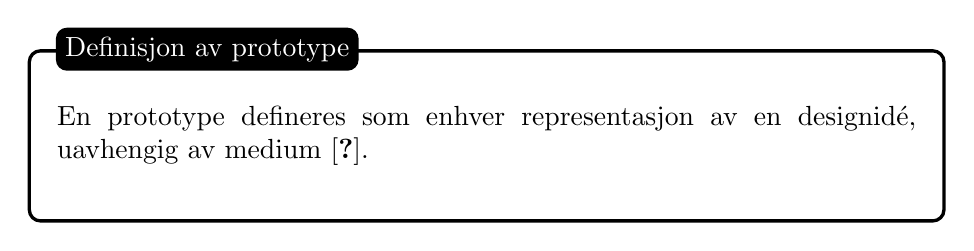
\begin{tikzpicture}
\node [mybox] (box){%
    \begin{minipage}{0.9\textwidth}
      En prototype defineres som enhver representasjon av en designidé, uavhengig av medium \cite{Houde97}.
    \end{minipage}
};
\node[fancytitle, rounded corners, right=10pt] at (box.north west) {Definisjon av prototype};
\end{tikzpicture}%


